\documentclass[12pt,a4paper]{article}
\usepackage[utf8]{inputenc}
\usepackage{amsmath}
\usepackage{geometry}
\usepackage{graphicx}
\usepackage{hyperref}
\usepackage{makeidx}

\usepackage{listings}
\usepackage{xcolor}
\usepackage{geometry}
 \geometry{
 a4paper,
 total={170mm,257mm},
 left=25mm,
 top=25mm,
 right = 25mm,
 bottom = 25mm
 }
\definecolor{codegreen}{rgb}{0,0.6,0}
\definecolor{codegray}{rgb}{0.5,0.5,0.5}
\definecolor{codepurple}{rgb}{0.58,0,0.82}
\definecolor{backcolour}{rgb}{0.95,0.95,0.92}

\lstdefinestyle{mystyle}{
    backgroundcolor=\color{backcolour},   
    commentstyle=\color{codegreen},
    keywordstyle=\color{magenta},
    numberstyle=\tiny\color{codegray},
    stringstyle=\color{codepurple},
    basicstyle=\ttfamily\footnotesize,
    breakatwhitespace=false,         
    breaklines=true,                 
    captionpos=b,                    
    keepspaces=true,                 
    numbers=left,                    
    numbersep=5pt,                  
    showspaces=false,                
    showstringspaces=false,
    showtabs=false,                  
    tabsize=2
}
\lstset{style=mystyle}
\makeindex
\begin{document}
	
\begin{titlepage}
	\begin{center}
		\vspace*{1cm}
		
		\LARGE
		\textbf{Interactive Graphics}
		
		\large 
		\textbf{Final Course Project}
		
		\vspace{1.5cm}
		Authors: \\
		Sveva Pepe - 1743997 \\ 
		Simone Tedeschi - 1762897 \\
		Claudia Medaglia - matricola \\
		Christian Marinoni - matricola
		\vfill
		
		
\includegraphics[width=0.7\textwidth]{logo}
	
		\vfill
		
		\large
		Professor: Marco Schaerf\break\break\break\break
		June 2020
		
	\end{center}
\end{titlepage}

\tableofcontents
\pagebreak
\section{Introduction}
The goal of the project is to implement an interactive application 
that make use of basic WebGL or advanced libraries, as in our case ThreeJS. The project 
cover the main aspects treated during the course, such as lights, textures, hierarchical models and animations.
\section{Game}
We decided to develop a 3D version of "Duck Hunt", a  
famous game from the 80s, in which the objective is to hit  
as many ducks as possible. We designed the
scene as a first-person game, where the player is located 
in a tall grass field and controls a rifle. 
Thanks to the help of his dog, that frighten the ducks hidden 
in the tall grass, the hunt can start. 
The game ends when the player miss five ducks.
In addition, our game provides other functionalities like enable 
and disable sounds, pause the game or restart it.
\\ \\The above described scene is depicted in the following figure:
\begin{figure}[hbt!]
    \centering
    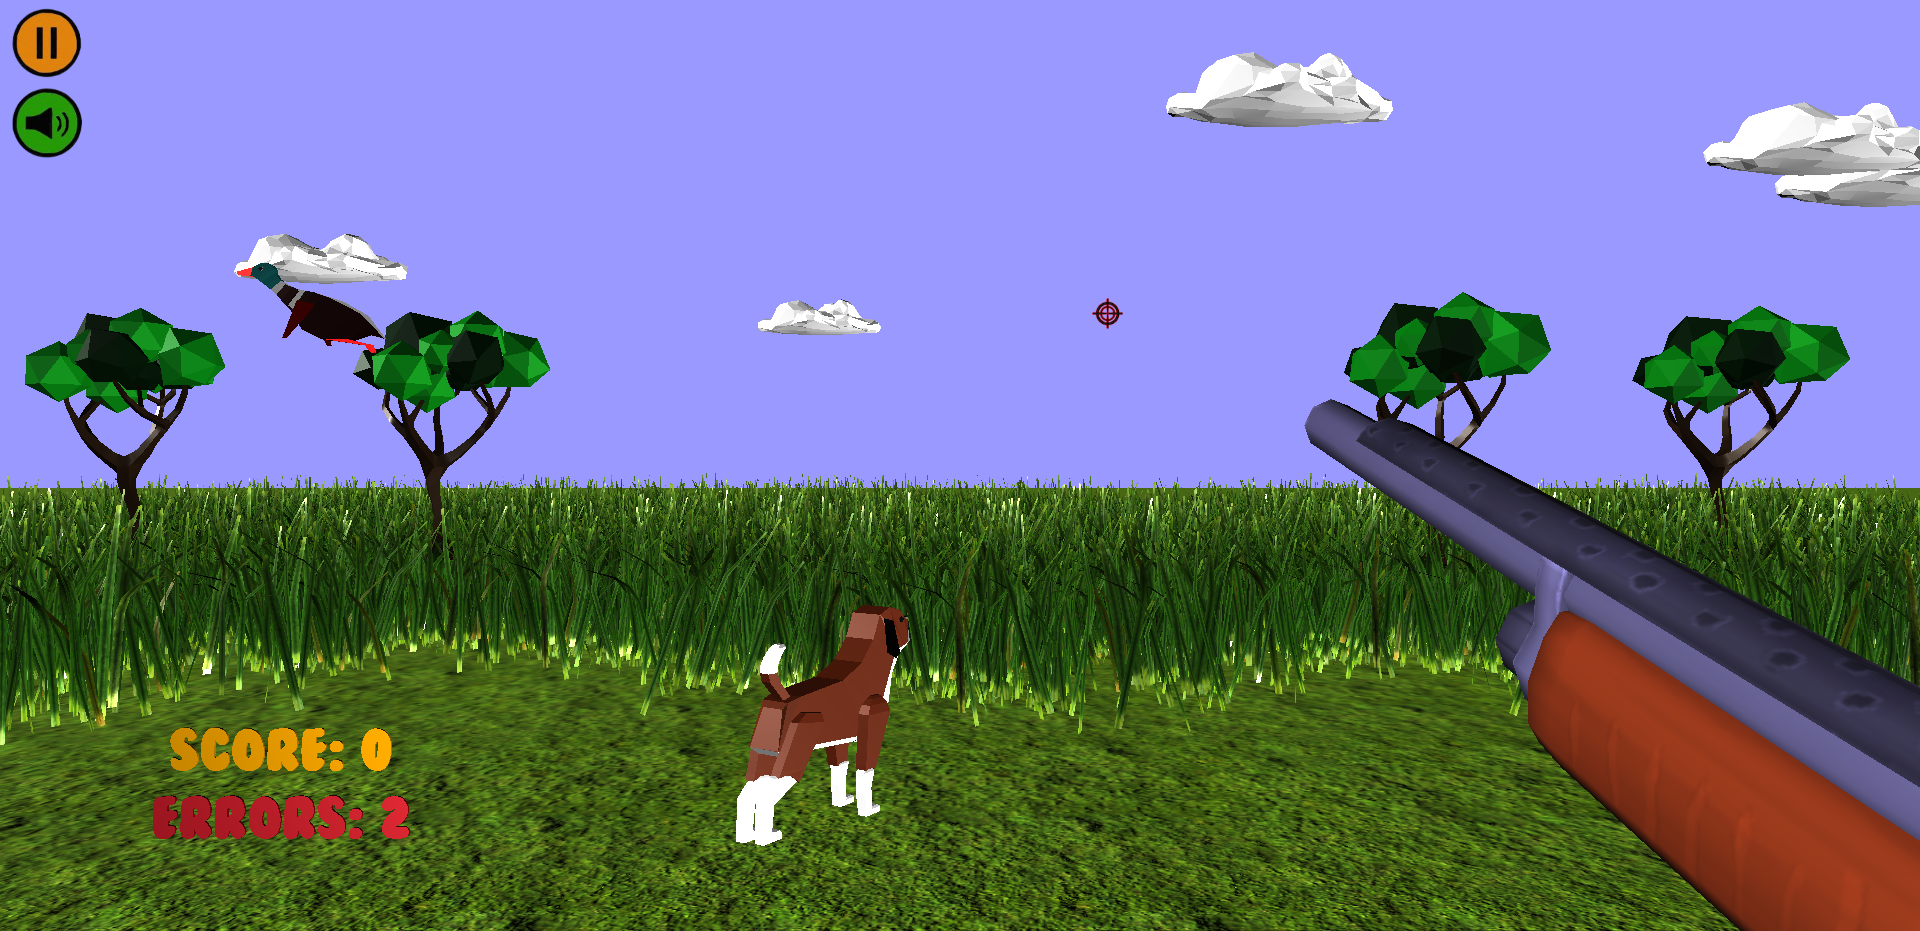
\includegraphics[width=1\textwidth]{game.png}
    \caption{Starting scene of the game.}
    \label{fig1}
\end{figure}
\section{Scene}
The scene shown in Figure \ref{fig1}, which is a ThreeJS object, 
has been obtained adding textures, lights, and different 3D models. 
The dog and the ducks are hand-made models while the other are 
taken from SketchFab. We used perspective camera to make the scene 
as realistic as possible to let the center of projection coincide 
with the user’s eyes.
The prospective uses as parameters: \textit{fovy, aspect, near and 
far}. \textit{Fovy}, which stands for "field of view y-axis",
identifies how wide the eyes open along the y direction.
\textit{Aspect} represent the ratio between the width and height
of the canvas.
\textit{Near} and \textit{far} are any positive numbers 
representing the minimum and maximum distances of the object, 
with the restriction that near is always less than far.
For the camera is defined also the  
\textit{lookAt(x, y, z)} method, where the \textit{x, y} and \textit{z} 
are the coordinates of the scene.
The texts on the bottom right corner instead, have beed modeled using
TTFLoader of ThreeJS, where through a Mesh the relative 
colors have been applied.
Moreover, in order to make our application responsive we add a 
dedicated Listener to adapt the window size based on the device
resolution. Finally, to improve the user experience antialiasing 
has been used.
\subsection{Lights and Textures}
The ground texture was created by repeatedly applying a texture on 
a plane, using a TextureLoader. Then, the texture is added to the
scene through the use of meshes that map texture coordinates into
world coordinates.
Three directional lights have also been added to the scene. 
Two of them were placed on the left upper and bottom right corner 
respectively of the scene to reproduce a sunny day, otherwise using
only one of them we obtain either dark clouds or dark objects. 
The third one has been introduced to illuminate texts because they 
are ahead of other elements and so the previous lights were
not able to light up also them.
\section{3D Models}
In this section we explain the models we have included in our project. They are splitted into
the following two categories: 
\begin{itemize}
\item linear models: objects that are treated as an atomic entity;
\item hierarchical models: objects composed by various sub-objects. 
\end{itemize}
\subsection{Linear Models} \label{linear}
The linear models are models that are treated as singles entities. In our game are present the following four groups of linear models: Rifle, Trees, Clouds and Bushes. They contain 1, 4, 5 and 11 instances respectively that can be observed in Figure \ref{fig1}. We did this categorization to handle different kinds of objects in different ways, because objects belonging to different groups are indipendent to each other. Trees/bushes positions and orientations have been preset and remain static along the entire gameplay. Clouds positions instead, vary over time and rifle orientation can be controlled by the user. These last two aspects will be further explained in Sections \ref{anim} and \ref{user} where we will provide technical details.
\subsection{Hierarchical Models}
Hierarchical models are models composed by different sub-objects that allow to represent relationships between such objects. The major benefit of hierarchical structures is the possibility to handle animations in a simple and efficient way, because, for instance, if we want to apply a rotation to the whole object we need only to perform it to the root of the object itself, instead of applying n rotations to each individual component.
\subsubsection{3D Duck Model}
The first hierarchical model that we introduced in our project is an hand-made 3D model of a duck, created with Blender. Its structure is divided into four components: left and right wings, torso (including also the head) and legs. Such structure allowed us to reproduce the desired behavior, which consists in a simultaneous diagonal translation and a synchronous upward rotation of the wings. The above described hiearchical structure is shown in the following figure:
\begin{figure}[hbt!]
	\centering
	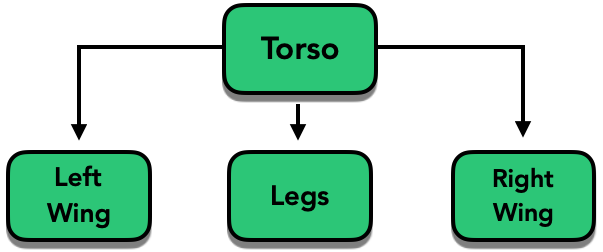
\includegraphics[width=0.7\textwidth]{hier_duck}
	\caption{Hierarchical model of the duck.}
	\label{fig2}
\end{figure}

\subsubsection{3D Dog Model}
The second hierarchical model that we used in our project is again an hand-made 3D model created with Blender, representing a dog. Its structure is divided into ten components: left and right upper front legs, left and right upper back legs, left and right lower front legs, left and right lower back legs, torso (including also the head) and tail. 
\\\\The hierarchical structure of the dog is depicted below: 
\begin{figure}[hbt!]
	\centering
	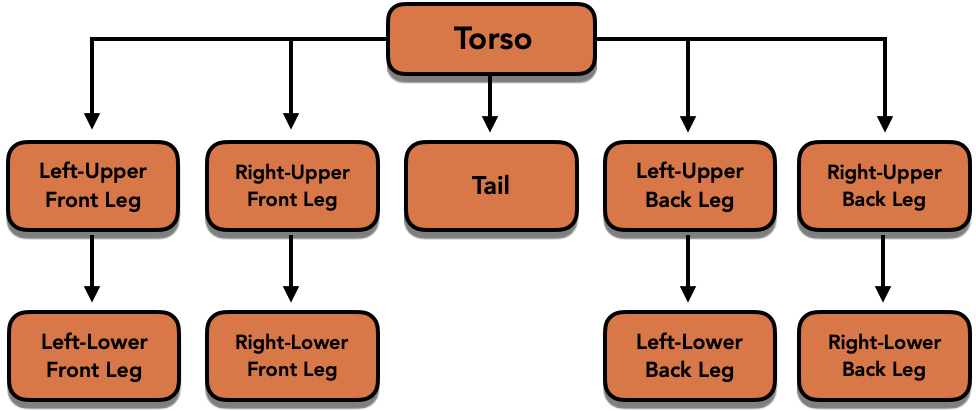
\includegraphics[width=0.98\textwidth]{hier_dog}
	\caption{Hierarchical model of the dog.}
	\label{fig3}
\end{figure}
\hfill \break We exploit such structure to let the dog move towards the bushes with few basic movements. To achieve this, we simply translate the "Torso" node, which is the root of the hierarchy tree, and automatically all other components, which are attached to it, will follow its movement. In the meanwhile, we alternate the legs movements back and forth to reproduce a walk. Additional details will be provided in the Animations section (\ref{anim}).

\section{Animations}\label{anim}
\section{User Interaction} \label{user}
\subsection{Sounds}
\section{Conclusion}
\end{document}